% hw1-regression.tex
\documentclass{article} %The basic layout of the output document, sets things like pagesize and defaults
\usepackage[authoryear,round]{natbib} %a package for formatting citations
\usepackage{amsmath} %a package for good looking equations and symbols
\usepackage{algorithm2e} %a package for typesetting algorithms
\usepackage{caption} %a package for more complex captions for figures/tables/images
\usepackage{subcaption} %extension of the caption package
\usepackage{url} %embedded, clickable links
\usepackage{fullpage} %including this package changes the default margins to use more of the page
\usepackage{graphicx} %package for inline images
\usepackage[usenames]{xcolor} %for adding color text
\usepackage{enumitem} %for nested numbered lists (like in the questions section)

\bibliographystyle{plainnat}

%note that the title and date are specified /before/ the "\begin{document}" command.
\title{CS 4641: Machine Learning\\ %double backslash (ie, "\\") are typically used to force a newline in most environments
Homework 1 --- Regression}
\date{} %an empty string "{}" is OK here, but some environments/commands will throw an error.
\author{}

\begin{document}
\maketitle %The "\maketitle command" is what actually formats and inserts this information into the text.

%some latex magic that creates a new command for use in this document. This particular command is handy for annotating
%changes or temporary text.
\newcommand{\bphnote}[1]{\textit{\textcolor{red}{#1}}}


\section*{Instructions} %Sections and subsections create headers and are automatically numbered
\subsection*{Submission}
Submission will be handled using Canvas, as will announcements regarding due dates or any changes to this assignment. 
All the assignments this semester will contain some coding and some written questions. In order to keep things reasonable for 
your TAs to grade, please submit \textbf{one} zipfile containing a folder with \textbf{all} your code, data files, and a 
\textbf{single} pdf with your answers to the written questions. This zipfile should have the following format: 
\texttt{hw1-GTusername.zip}, replacing ``GTusername'' with your username (for example ``hw1-bhrolenok3.zip'').

%One of the more common environments are "enumerate" or "itemize" which create numbered or bulletized lists respectively.
For this assignment, your submission should include:
\begin{itemize}
	\item \texttt{hw1-answers.pdf} A PDF of your answers to the written questions. You can use whatever software you like to create your report, but what you turn in must be a PDF (no .docx, .txt, .rtf...). We recommend \LaTeX~(which is how this handout was created) because it generates professional looking reports, and is a good tool to learn. For a simple example, the source that generated this file is included with the template code.
	\item \texttt{hw1.py} The template file, modified to include your code.
	\item \texttt{README} Any special instructions for running your code, (library versions, network access, etc) \textbf{plus}
	any external sources you used to help you with this assignment. This includes other students and websites. When in doubt, cite it!
\end{itemize}

\subsection*{Collaboration}
All of the assignments in this class are \textbf{individual work only}. You're welcome to \emph{discuss} the math or high 
level concepts behind the algorithms you're being asked to implement, but you are 
\textbf{not allowed to share code or answers to the written questions}. We will be checking, manually and with automated 
tools, for any violations of this policy, so please \textbf{do not share solutions or code}.

\section*{Coding}
Linear regression is probably one of the simplest and yet most widely used learning algorithms that we'll discuss in this 
class. Partly, this is because it is an extremely simple algorithm, both to implement and to analyze, which is why it's a 
good place to start! In the rest of this exercise, you'll implement linear regression several different ways, and explore a 
simple but powerful extension.

\subsection*{Setting up and code template}
A short template has been provided for you in the file \texttt{hw1.py}. The only dependencies are 
NumPy\footnote{\url{https://numpy.org/}} and matplotlib\footnote{\url{https://matplotlib.org}}, and these are fairly 
straightforward libraries to install on any system, Linux, Mac, and Windows. You can use whatever development environment you 
wish, but we recommend something simple, like your favorite text editor, the command line, and 
\texttt{virtualenv}\footnote{\url{https://virtualenv.pypa.io/}}.

Once you think you've got everything set up, you can test by running \texttt{hw1.py} from the command line. This should 
display the \texttt{data/2D-noisy-lin.txt} as a 3D scatter plot, which should look like Figure \ref{test-plot-fig}. If you 
encounter any errors, or the figure looks significantly different, debug your installation first since the rest of this 
assignment depends on these libraries.

After getting everything working, start digging in to the code in the template. Most functions are thoroughly commented, even 
those you don't need to modify to complete the assignment. You might find some snippets that are useful elsewhere in the assignment, or for future assignments.

\begin{figure}
\begin{center}
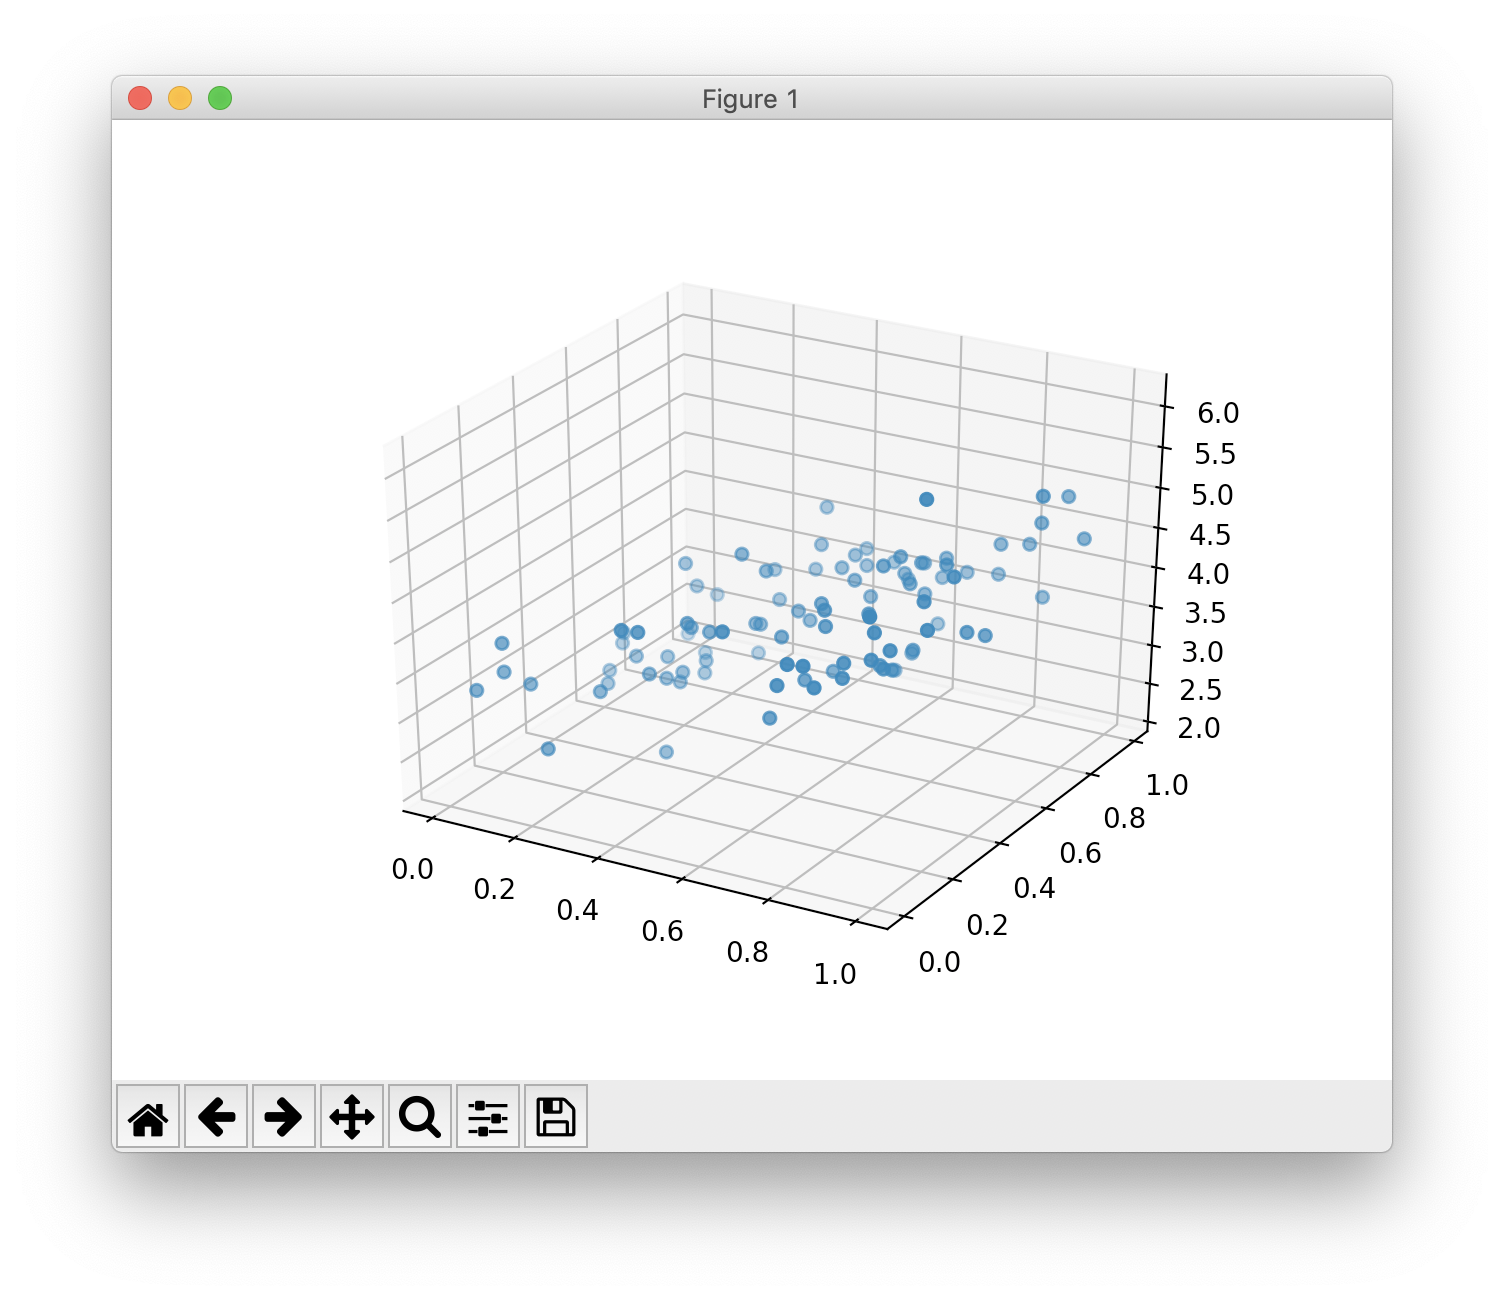
\includegraphics[height=0.5\textheight]{test-plot}
\caption{The what the demo output should look like.}
\label{test-plot-fig}
\end{center}
\end{figure}

\subsection*{Linear Regression - closed form solution}
Now you should be ready to implement Linear Regression. First, recall the equation for our general linear model in 
matrix/vector notation
\begin{align*}
	h_\theta(\mathbf{x}) &= \mathbf{x}^\top \theta 
\end{align*}
%
where we're using convention that \(x_0 = 1\) (we prepend \(1\) to our feature vector). This tells us how to use \(\theta\) 
to predict \(y\) for a given \(x\). To actually find \(\theta\) we can construct a system of linear equations out of our 
training data like so: 
\begin{align*}
	\mathbf{X} &= \left[\begin{array}{cccc} x^{(1)}_0 & x^{(1)}_1 & \cdots & x^{(1)}_D\\ x^{(2)}_0 & x^{(2)}_1 & \cdots & x^{(2)}_D\\ \vdots & & \ddots & \\ x^{(N)}_0 & x^{(N)}_1 & \cdots & x^{(N)}_D\end{array}\right] = \left[\begin{array}{ccc}\text{---}&\mathbf{x}^{(1)\top}&\text{---}\\ \text{---}&\mathbf{x}^{(2)\top}&\text{---}\\ &\vdots&\\\text{---}&\mathbf{x}^{(N)\top}&\text{---}\end{array}\right]\\
	\mathbf{y} &= \left[\begin{array}{c}y^{(1)}\\ y^{(2)}\\ \vdots\\ y^{(N)} \end{array}\right]\\
	\mathbf{y} &= \mathbf{X} \theta
\end{align*}
%
which we can use to find an estimate for the parameters, \(\hat{\theta}\):
\begin{align}
	\hat{\theta} &= \left(\mathbf{X}^\top \mathbf{X}\right)^{-1} \mathbf{X}^\top \mathbf{y} \label{eqn:closed-form}
\end{align}

Note that since this is just a bunch of matrix multiplications, transposes, and one matrix inverse, we can actually code this
as a single line using numpy, although you can break it out into multiple steps to make it obvious and easier to debug. Look 
at the documentation for \texttt{numpy.dot(...)}, \texttt{numpy.transpose(...)}, and \texttt{numpy.linalg.inv(...)}, play 
around with them for simple 2-by-2 matrices until you understand them, then use them to build up equation 
\ref{eqn:closed-form} in the function \texttt{linreg\_closed\_form(...)}. You can test your work on the provided datasets or 
data you make yourself, and compare with the results that \texttt{numpy.linalg.lstsq(...)} produces. (Note: to get credit for 
this part be sure to actually implement the equation, don't use the output of \texttt{numpy.linalg.lstsq(...)}). You can also 
visualize the model you are finding with the \texttt{vis\_linreg\_model(...)} function.

\subsection*{Gradient Descent}
What happens when we have a lot of data points or a lot of features? Notice we're computing 
\(\left(\mathbf{X}^\top\mathbf{X}\right)^{-1}\) 
which becomes computationally expensive as that matrix gets larger. In the section after this we're going to need to be able 
to compute the solution for some really large matrices, so we're going to need a method that doesn't compute this inverse.

Gradient Descent is one such method, one that's used in a variety of algorithms in ML. The basic outline of the gradient 
descent method is to ``follow'' the gradient of the loss function, \(\nabla_\theta \mathcal{J}_S(h_\theta)\), to a minimum for the 
parameters, \(\theta\). First lets define the loss function as the squared-loss:
\begin{align}
	\mathcal{J}_S(h_\theta) &= \frac{1}{2N} \sum_{i=1}^N \left(h_\theta(\mathbf{x}^{(i)})-\mathbf{y}^{(i)}\right)^2 \label{eqn:loss}
\end{align}

Implement equation \ref{eqn:loss} in the function \texttt{loss(...)}. You can check that it works by using 
\texttt{numpy.linalg.lstsq(...)} on the provided datasets. Note that the residuals returned by 
\texttt{numpy.linalg.lstsq(...)} are the sum of squared errors, so you will have to scale appropriately.

We can use Gradient Descent on this loss function to find the optimal parameters for our linear model by iteratively updating 
\(\theta\), adding in a small bit of the negative of the gradient. Here's a formal description of the algorithm:

\begin{algorithm}[H]
	\SetAlgoLined
	\KwData{initial estimate \(\hat{\theta}^{(0)}\), loss function \(\mathcal{J}_S(h_\theta)\), number of iterations \(K\), learning rate \(\alpha\)}
	\KwResult{estimate of optimal parameters, \(\hat{\theta}^{(K)}\)}
	\For{\(k\leftarrow 1\) \KwTo \(K\)}{
		\(\hat{\theta}^{(k)} \leftarrow \hat{\theta}^{(k-1)} - \alpha \nabla \mathcal{J}_S(\hat{\theta}^{(k-1)})\)
	}
\end{algorithm}

As we showed in class, for our linear model and using equation \ref{eqn:loss} for the loss, we can write the gradient as:
\begin{align}
	\nabla \mathcal{J}_S(h_\theta) = \frac{1}{N}\left(\mathbf{X}^\top\mathbf{X}\theta -\mathbf{X}^\top\mathbf{Y}\right) \label{eqn:gradient}
\end{align}

Implement Gradient Descent using equation \ref{eqn:gradient} in the function \texttt{linreg\_grad\_desc(...)}. You can check 
that it works by comparing your answers for the closed form solution or \texttt{numpy.linalg.lstsq(...)}. The default values 
for \texttt{alpha} and \texttt{num\_iters} should be enough for gradient descent to converge to the same answers for the 
linear datasets, but you may want to test for higher or lower values to see how it affects the results. Again, it will 
probably be helpful to use \texttt{vis\_linreg\_model(...)} to visualize the resulting models.

\subsection*{Random Fourier Features}

Linear Regression, unsurprisingly enough, can only fit \textbf{linear} data with any degree of accuracy. However, as we 
discussed in the class it's fairly easy to extend Linear Regression by transforming the data using a set of \(K\) non-linear 
feature functions, which we'll denote \(\Phi=\{\phi_k(\mathbf{x})\}_{k=1}^K\).

There are many possible ways to choose the set \(\Phi\)\footnote{and if you have any insight into the kinds of functions that 
generated your training data, it's a good idea to start with those.}, but there are actually a few methods that extend Linear 
Regression to fit models from almost any class of functions. One particularly simple (to implement) method is called 
\emph{Random Fourier Features} which is described by \citet{rff-cite}. The key idea is that any ``well behaved'' function can 
be represented by its Fourier transform, which is basically a sum of an infinite number of \(\sin\) and \(\cos\) functions 
with different amplitudes and frequencies. The trick is that we can \emph{approximate} this infinite sum with a \emph{finite} 
number of samples, as long as we sample appropriately at randomly selected frequencies. The way this is implemented is by 
using the following set of basis functions:
% \begin{align*}
% 	f(x) &= \int_0^\infty a(\lambda) \cos(2\pi\lambda x) + b(\lambda) \sin(2\pi\lambda x) d\lambda\\
% 	% f(x) = \sum_{n=-\infty}^\infty c_n e^{2\pi i \left(\frac{n}{T}\right)x} &= \left(\sum_{n=-\infty}^\infty c_n\left(\cos\left(2\pi\frac{n}{T}x\right) + i \sin\left(2\pi\frac{n}{T}x\right)\right)\right)\\
% 	&\approx \sum_{k=1}^{K} \theta_k\left(\cos\left(\omega_k x + b_k\right)\right)
% \end{align*}
\begin{align*}
	\phi_k(\mathbf{x}) &= \cos(\omega_k x + b_k),~~~~k=1,\ldots,K
\end{align*}

So using using this set of basis functions, and randomly selecting \(\omega_k\) and \(b_k\), gives us a problem that's linear 
in the features (so we can use linear regression), and which should let us fit \emph{almost} any function (where \emph{almost}
includes any function for which the Fourier inversion theorem holds). 
This also means that as we add more and more features (as we increase \(K\)), we should be able to more and more accurately 
estimate any crazy non-linear function we like! The proof that this is true, and the  details of how exactly to do this 
sampling for \(\omega_k\) and \(b_k\) are in the cited paper, which you'll need to read in order to implement the function 
\texttt{random\_fourier\_features(...)}. The paper gives different ways of sampling for different ``kernels;'' we'll talk 
about these in more detail later, but for now use the method for the Gaussian kernel. 

The math in the paper may be a bit advanced, but the actual code that you have to write is minimal (less than 5 lines total), 
as a lot has been filled in for you, there and in the helper functions. Perhaps the most complicated part is getting the 
shape of the matrix right for the helper funciton \texttt{apply\_RFF\_transform(...)} to work with the code as written. The 
helper function is expecting a 1D array for 
\(\mathbf{b}\) and a D-by-K matrix for the \(\omega\)'s:
\begin{align*}
	% \mathbf{b} &= \left[\begin{array}{c}b_1\\b_2\\\vdots\\b_K\end{array}\right]\\
	\Omega &= \left[\begin{array}{cccc}\vrule&\vrule& &\vrule\\\omega_1&\omega_2&\cdots&\omega_K\\\vrule&\vrule& &\vrule\end{array}\right]
\end{align*}

The comments in that function also have good pointers for which \texttt{numpy} methods you'll want to use for the sampling.

\subsubsection*{A note about testing RFF}
Since you are randomly sampling the transform for Random Fourier Features, your results may vary from one run to the next. Be 
sure to test your work, using the provided non-linear datasets like \texttt{1D-exp-*.txt} and \texttt{1D-quad-*.txt}, 
multiple times to get a good idea of how this method performs. As with gradient descent, the default parameters should 
produce reasonable results, but you will want to change these settings to get a good feel for what's going on, as well as to 
help with debugging.

\section*{Questions}
\begin{enumerate}
	\item Linear Regression
	\begin{enumerate}
		\item Use your closed form implementation to fit a model to the data in \texttt{1D-no-noise-lin.txt} and 
		\texttt{2D-noisy-lin.txt}. What is the loss of the fit model in both cases? Include plots for both. Note: for some of 
		these datasets the y-intercept will be non-zero, make sure you handle this case!
		\item What happens when you're using the closed form solution and one of the features (columns of \(\textbf{X}\)) is 
		duplicated? Explain why. Note: you may want to test this out with your code as a useful \emph{first step}, but you should think critically about what is happening and why.
		\item Does the same thing happen if one of the training points (rows of \(\textbf{X}\)) is duplicated? Explain why.
		\item Does the same thing happen with Gradient Descent? Explain why.
	\end{enumerate}
	\item Gradient Descent
	\begin{enumerate}
		\item Now use your Gradient Descent implementation to fit a model to \texttt{1D-no-noise-lin.txt} with 
		\texttt{alpha=0.05}, \texttt{num\_iters=10}, and \texttt{initial\_Theta} set to the zero vector. What is the output 
		(the full list of (\(\theta\), loss) tuples for each of the 10 iterations)?
		
		\item Using the default parameters for \texttt{alpha} and \texttt{num\_iters}, and with \texttt{initial\_Theta} set to 
		\(\mathbf{0}\), do you get the same model parameters as you did with the closed form solution? the same loss? Report this for both \texttt{1D-no-noise-lin.txt} and \texttt{2D-noisy-lin.txt}.
		
		\item Find a set of values of the learning rate and iterations where you get the same answers and a set of values 
		where the answers are noticeably different. Explain what's going on in both cases, and for both datasets \texttt{1D-no-noise-lin.txt} and \texttt{2D-noisy-lin.txt}.
	\end{enumerate}
	\item Random Fourier Features
	\begin{enumerate}
		\item Use your Random Fourier Features implementation to fit models for \texttt{1D-exp-samp.txt}, 
		\texttt{1D-exp-uni.txt}, \texttt{1D-quad-uni.txt}, and \texttt{1D-quad-uni-noise.txt}, each with 3 different values 
		for \(K\): small, medium, and large. The small value should noticeably under-fit the data, the large value should fit 
		almost perfectly, and the medium value should be somewhere in between. Report the values for \(K\) and include graphs 
		for each of the four datasets (so you should report 12 values of \(K\) and have 12 graphs in total).

		\item \textbf{EXTRA CREDIT}: What happens with Random Fourier Features if you try to predict a value far away from 
		any points in the training dataset? Modify the plotting functions (or write your own) and show what the model looks 
		like far away from the training points. Describe what you are seeing qualitatively, compare the model's output with 
		the ``true'' output quantitatively, and explain why this is happening. You may want to run these experiments multiple 
		times to get a better understanding of what is going on.
	\end{enumerate}
\end{enumerate}

\begin{thebibliography}{1}

\bibitem[Rahimi and Recht(2008)]{rff-cite} Rahimi, Ali, and Benjamin Recht. ``Random features for large-scale kernel 
machines.'' Advances in neural information processing systems. 2008.
\end{thebibliography}
\end{document}